\documentclass[]{article}
\usepackage{lmodern}
\usepackage{amssymb,amsmath}
\usepackage{ifxetex,ifluatex}
\usepackage{fixltx2e} % provides \textsubscript
\ifnum 0\ifxetex 1\fi\ifluatex 1\fi=0 % if pdftex
  \usepackage[T1]{fontenc}
  \usepackage[utf8]{inputenc}
\else % if luatex or xelatex
  \ifxetex
    \usepackage{mathspec}
  \else
    \usepackage{fontspec}
  \fi
  \defaultfontfeatures{Ligatures=TeX,Scale=MatchLowercase}
\fi
% use upquote if available, for straight quotes in verbatim environments
\IfFileExists{upquote.sty}{\usepackage{upquote}}{}
% use microtype if available
\IfFileExists{microtype.sty}{%
\usepackage{microtype}
\UseMicrotypeSet[protrusion]{basicmath} % disable protrusion for tt fonts
}{}
\usepackage[margin=1in]{geometry}
\usepackage{hyperref}
\hypersetup{unicode=true,
            pdfborder={0 0 0},
            breaklinks=true}
\urlstyle{same}  % don't use monospace font for urls
\usepackage{graphicx,grffile}
\makeatletter
\def\maxwidth{\ifdim\Gin@nat@width>\linewidth\linewidth\else\Gin@nat@width\fi}
\def\maxheight{\ifdim\Gin@nat@height>\textheight\textheight\else\Gin@nat@height\fi}
\makeatother
% Scale images if necessary, so that they will not overflow the page
% margins by default, and it is still possible to overwrite the defaults
% using explicit options in \includegraphics[width, height, ...]{}
\setkeys{Gin}{width=\maxwidth,height=\maxheight,keepaspectratio}
\IfFileExists{parskip.sty}{%
\usepackage{parskip}
}{% else
\setlength{\parindent}{0pt}
\setlength{\parskip}{6pt plus 2pt minus 1pt}
}
\setlength{\emergencystretch}{3em}  % prevent overfull lines
\providecommand{\tightlist}{%
  \setlength{\itemsep}{0pt}\setlength{\parskip}{0pt}}
\setcounter{secnumdepth}{0}
% Redefines (sub)paragraphs to behave more like sections
\ifx\paragraph\undefined\else
\let\oldparagraph\paragraph
\renewcommand{\paragraph}[1]{\oldparagraph{#1}\mbox{}}
\fi
\ifx\subparagraph\undefined\else
\let\oldsubparagraph\subparagraph
\renewcommand{\subparagraph}[1]{\oldsubparagraph{#1}\mbox{}}
\fi

%%% Use protect on footnotes to avoid problems with footnotes in titles
\let\rmarkdownfootnote\footnote%
\def\footnote{\protect\rmarkdownfootnote}

%%% Change title format to be more compact
\usepackage{titling}

% Create subtitle command for use in maketitle
\newcommand{\subtitle}[1]{
  \posttitle{
    \begin{center}\large#1\end{center}
    }
}

\setlength{\droptitle}{-2em}

  \title{}
    \pretitle{\vspace{\droptitle}}
  \posttitle{}
    \author{}
    \preauthor{}\postauthor{}
    \date{}
    \predate{}\postdate{}
  

\begin{document}

\textbf{8. Figures}

Figure 1. Plot photographs taken from study block 4 in King's River
Valley, west of Orovada, Nevada. We show these to illustrate the
apparent similarity between plots with different fire frequencies, and
why we thought species composition would not change dramatically between
one and 3 fires, while also hypothesizing that diversity would decline.

Figure 2. The extent of the study area is shown in (A). The striping
from the scanner line correction failure from Landsat 7 is clearly
visible and those areas were avoided in our sampling. Darker shading
indicates higher fire frequency. The potential range is 0 to 5 fires,
although areas with more than 3 fires were extremely rare (0.2\% of
total area). We sampled frequencies 0 to 3. The placement of the study
area within the Central Basin and Range ecoregion is shown in (B). A
detail of one of the study blocks is represented in (C).

Figure 3. Ordination plot of non-metric multidimensional scaling
conducted on plant community data using Kulcynski hierarchical
clustering. Ellipses represent the 95\% confidence interval around plots
grouped by whether or not they had burned. Species significantly (p
\textless{} 0.05) correlated with the ordination are shown, with arrows
scaled by the strength of the correlation. Species are listed by their
USDA plant codes. ARTRW8 is \emph{Artemisia tridentata} ssp.
\emph{wyomingensis}; POSE is \emph{Poa secunda}; ELEL5 is \emph{Elymus
elymoides}; SIAL2 is \emph{Sisymbrium altissimum}; BRTE is \emph{Bromus
tectorum}; CETE5 is \emph{Ceratocephalum testiculatum}; ERCI6 is
\emph{Erodium cicutarium}.

Figure 4. Alpha Diversity (Shannon's index of proportional abundance,
Pielou's index of evenness, and the number of species per plot), Beta
Diversity (Whittaker's index - the values are a unitless index of
dissimiliarity), and native and exotic plant cover, all grouped by fire
frequency. Shading indicates significantly different groups as
determined by Tukey's test.

Figure 5. Percent cover of life form groups, grouped by fire frequency.
Of the two most dominant life form groups, exotic annual grass is
\textgreater{}99\% cheatgrass, and native shrub is \textgreater{}99\%
Wyoming big sagebrush.

Figure 6. Species accumulation curves for fire frequency. Vertical lines
represent the conditioned standard deviation around species richness,
and are jittered for visibility.

Figure 7. Scatter plots for diversity indexes as predicted by
\emph{Bromus tectorum} cover and elevation. Lines are predictions from
linear mixed effects models with study block as a random effect. The X
axis is cheatgrass cover, and the Y axis is the value of the index with
the effect of elevation removed (Hohenstein 2018).

\newpage

\begin{figure}
 
  \begin{center}
    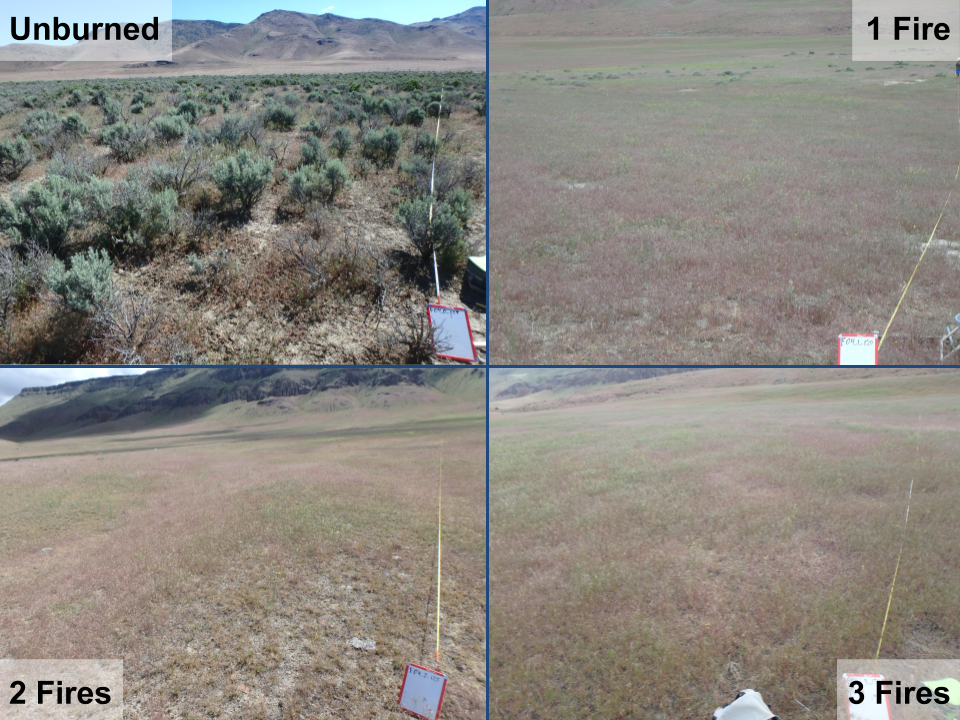
\includegraphics{figures/fire_pics.png}
    \caption{}
  \end{center}
\end{figure}

\clearpage

\newpage

\begin{figure}
 
  \begin{center}
    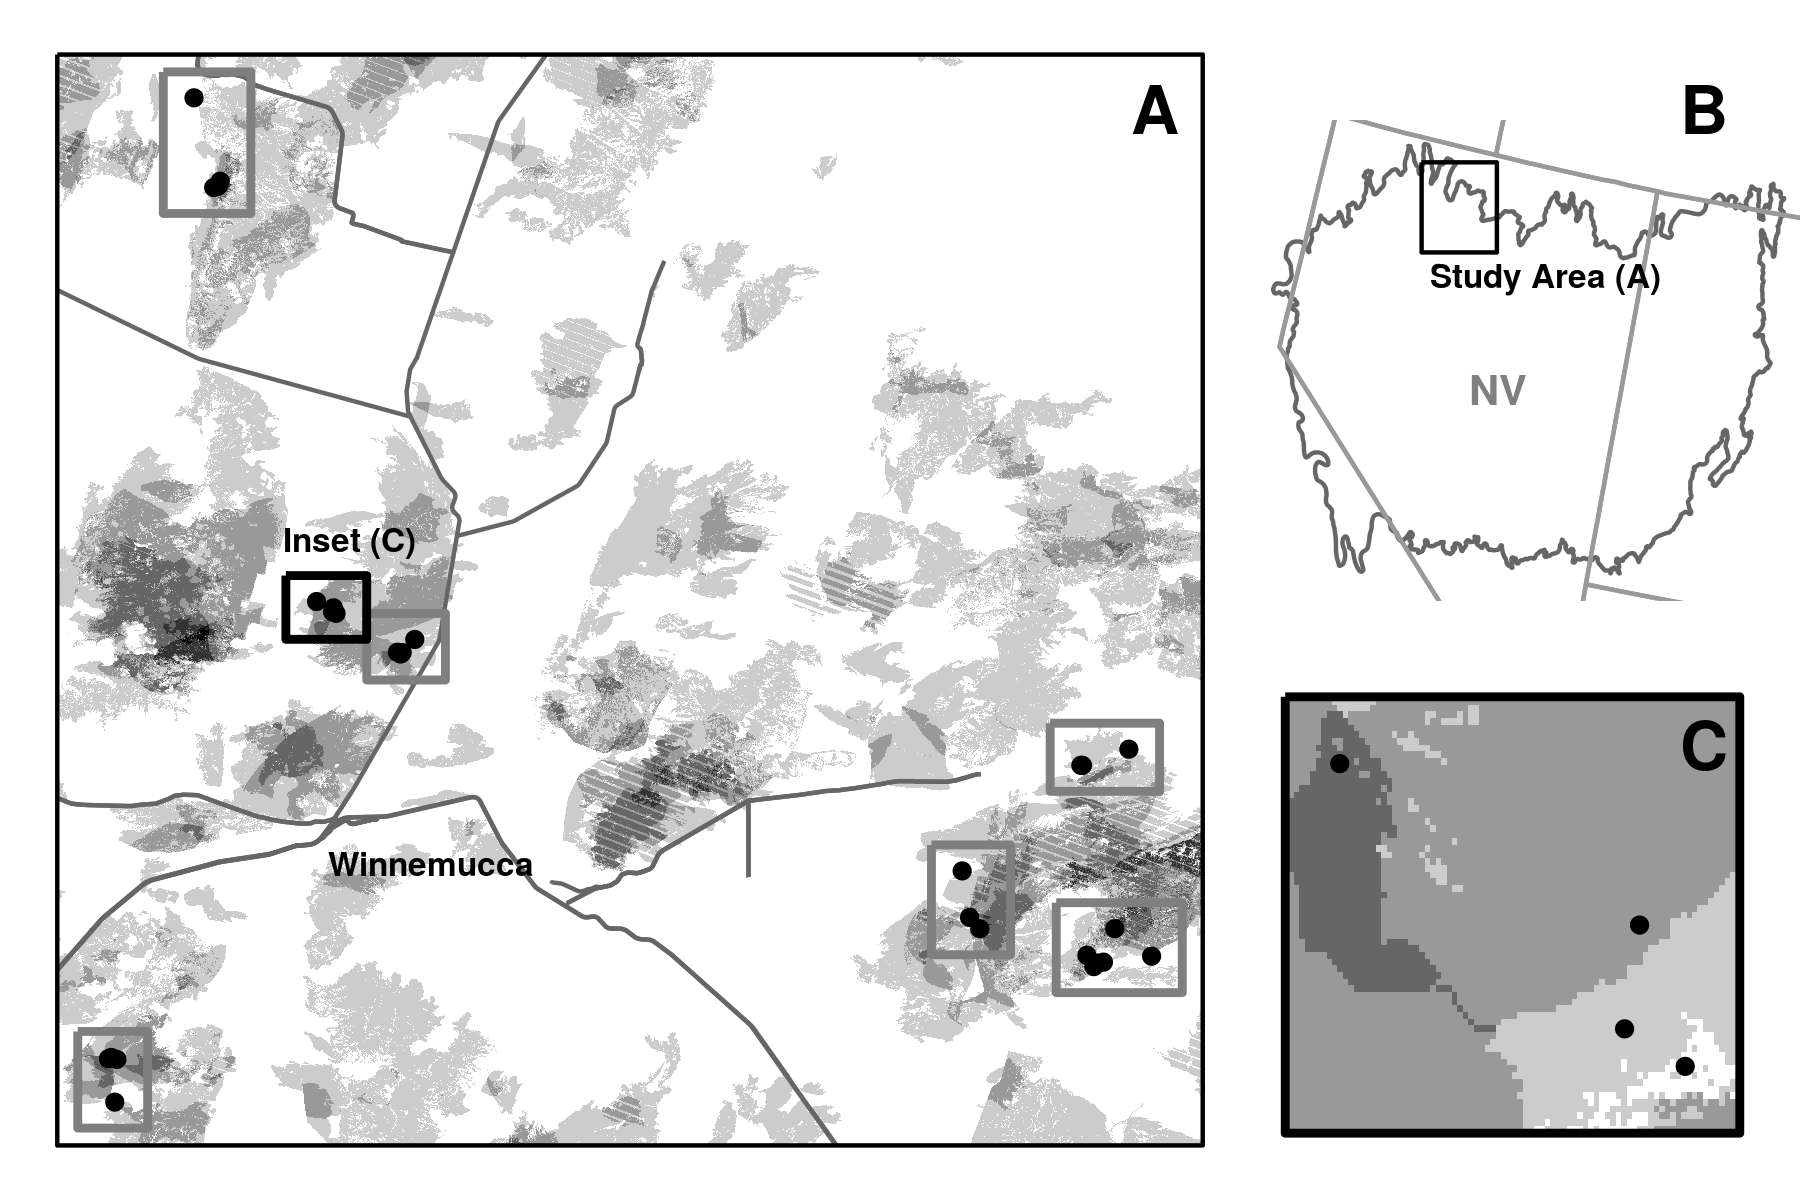
\includegraphics{figures/map.png}
    \caption{}
  \end{center}
\end{figure}

\clearpage

\newpage

\begin{figure}
 
  \begin{center}
    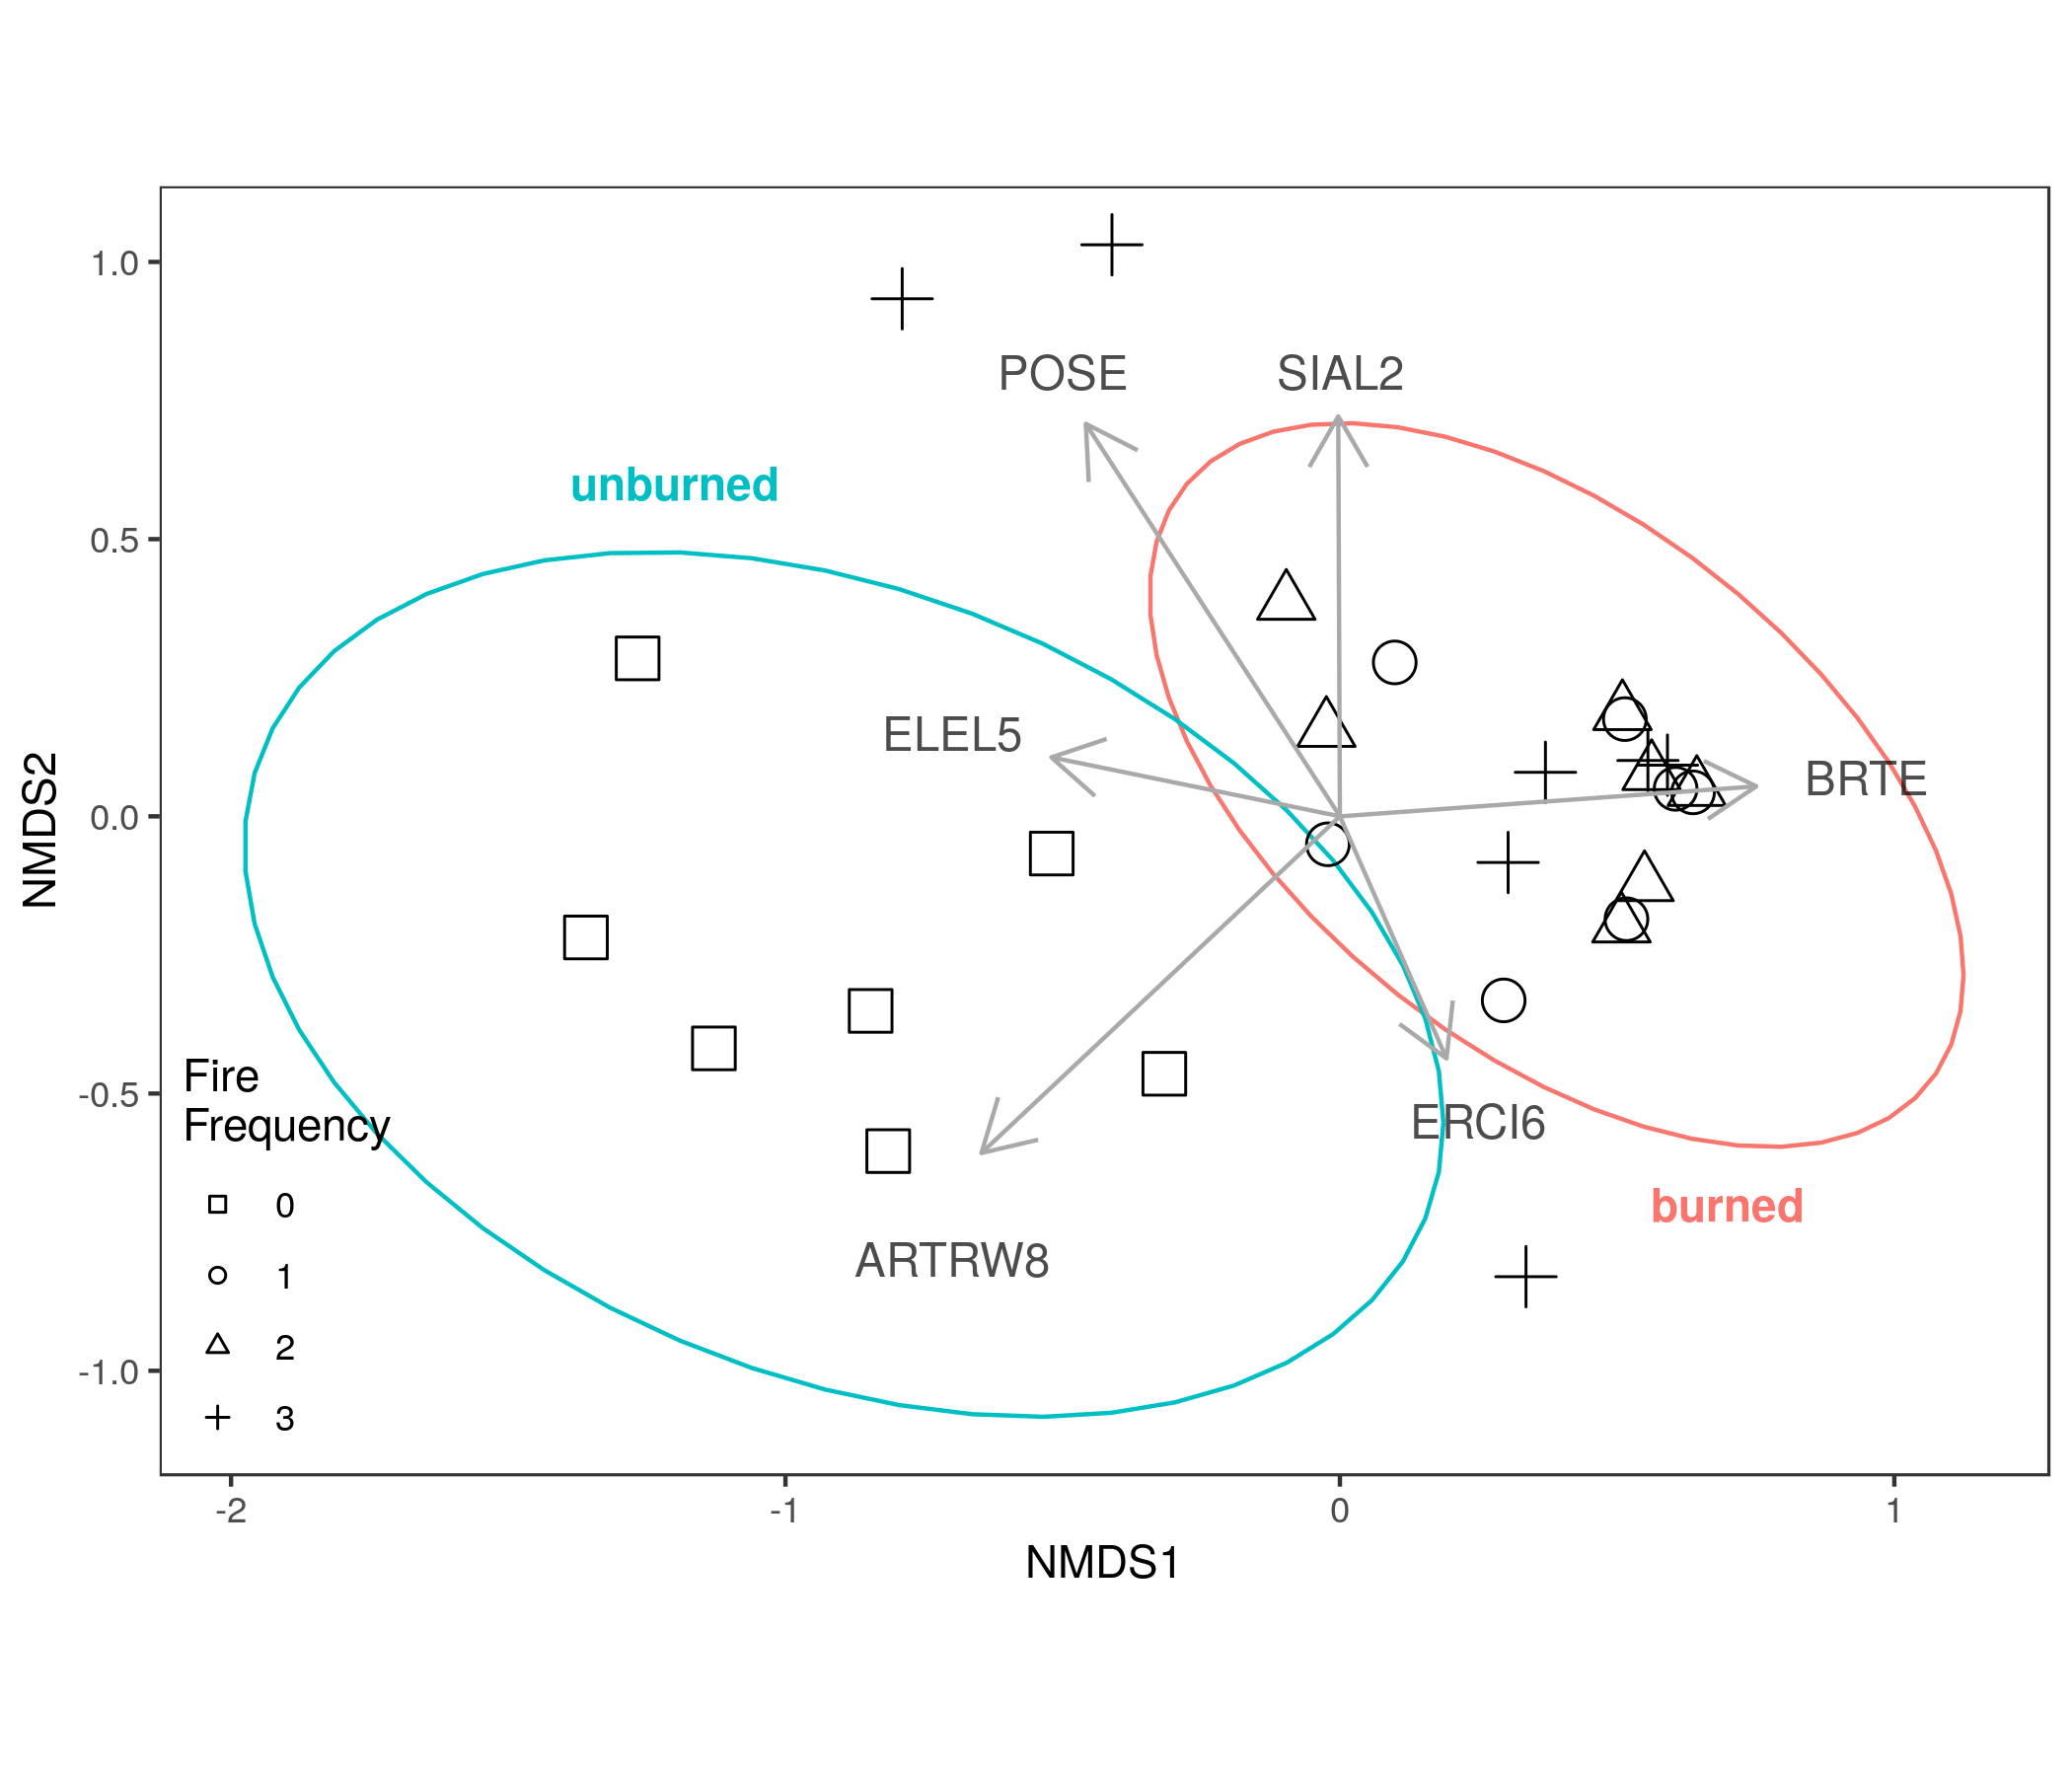
\includegraphics{figures/nmds.png}
    \caption{}
  \end{center}
\end{figure}

\clearpage

\newpage

\begin{figure}
 
  \begin{center}
    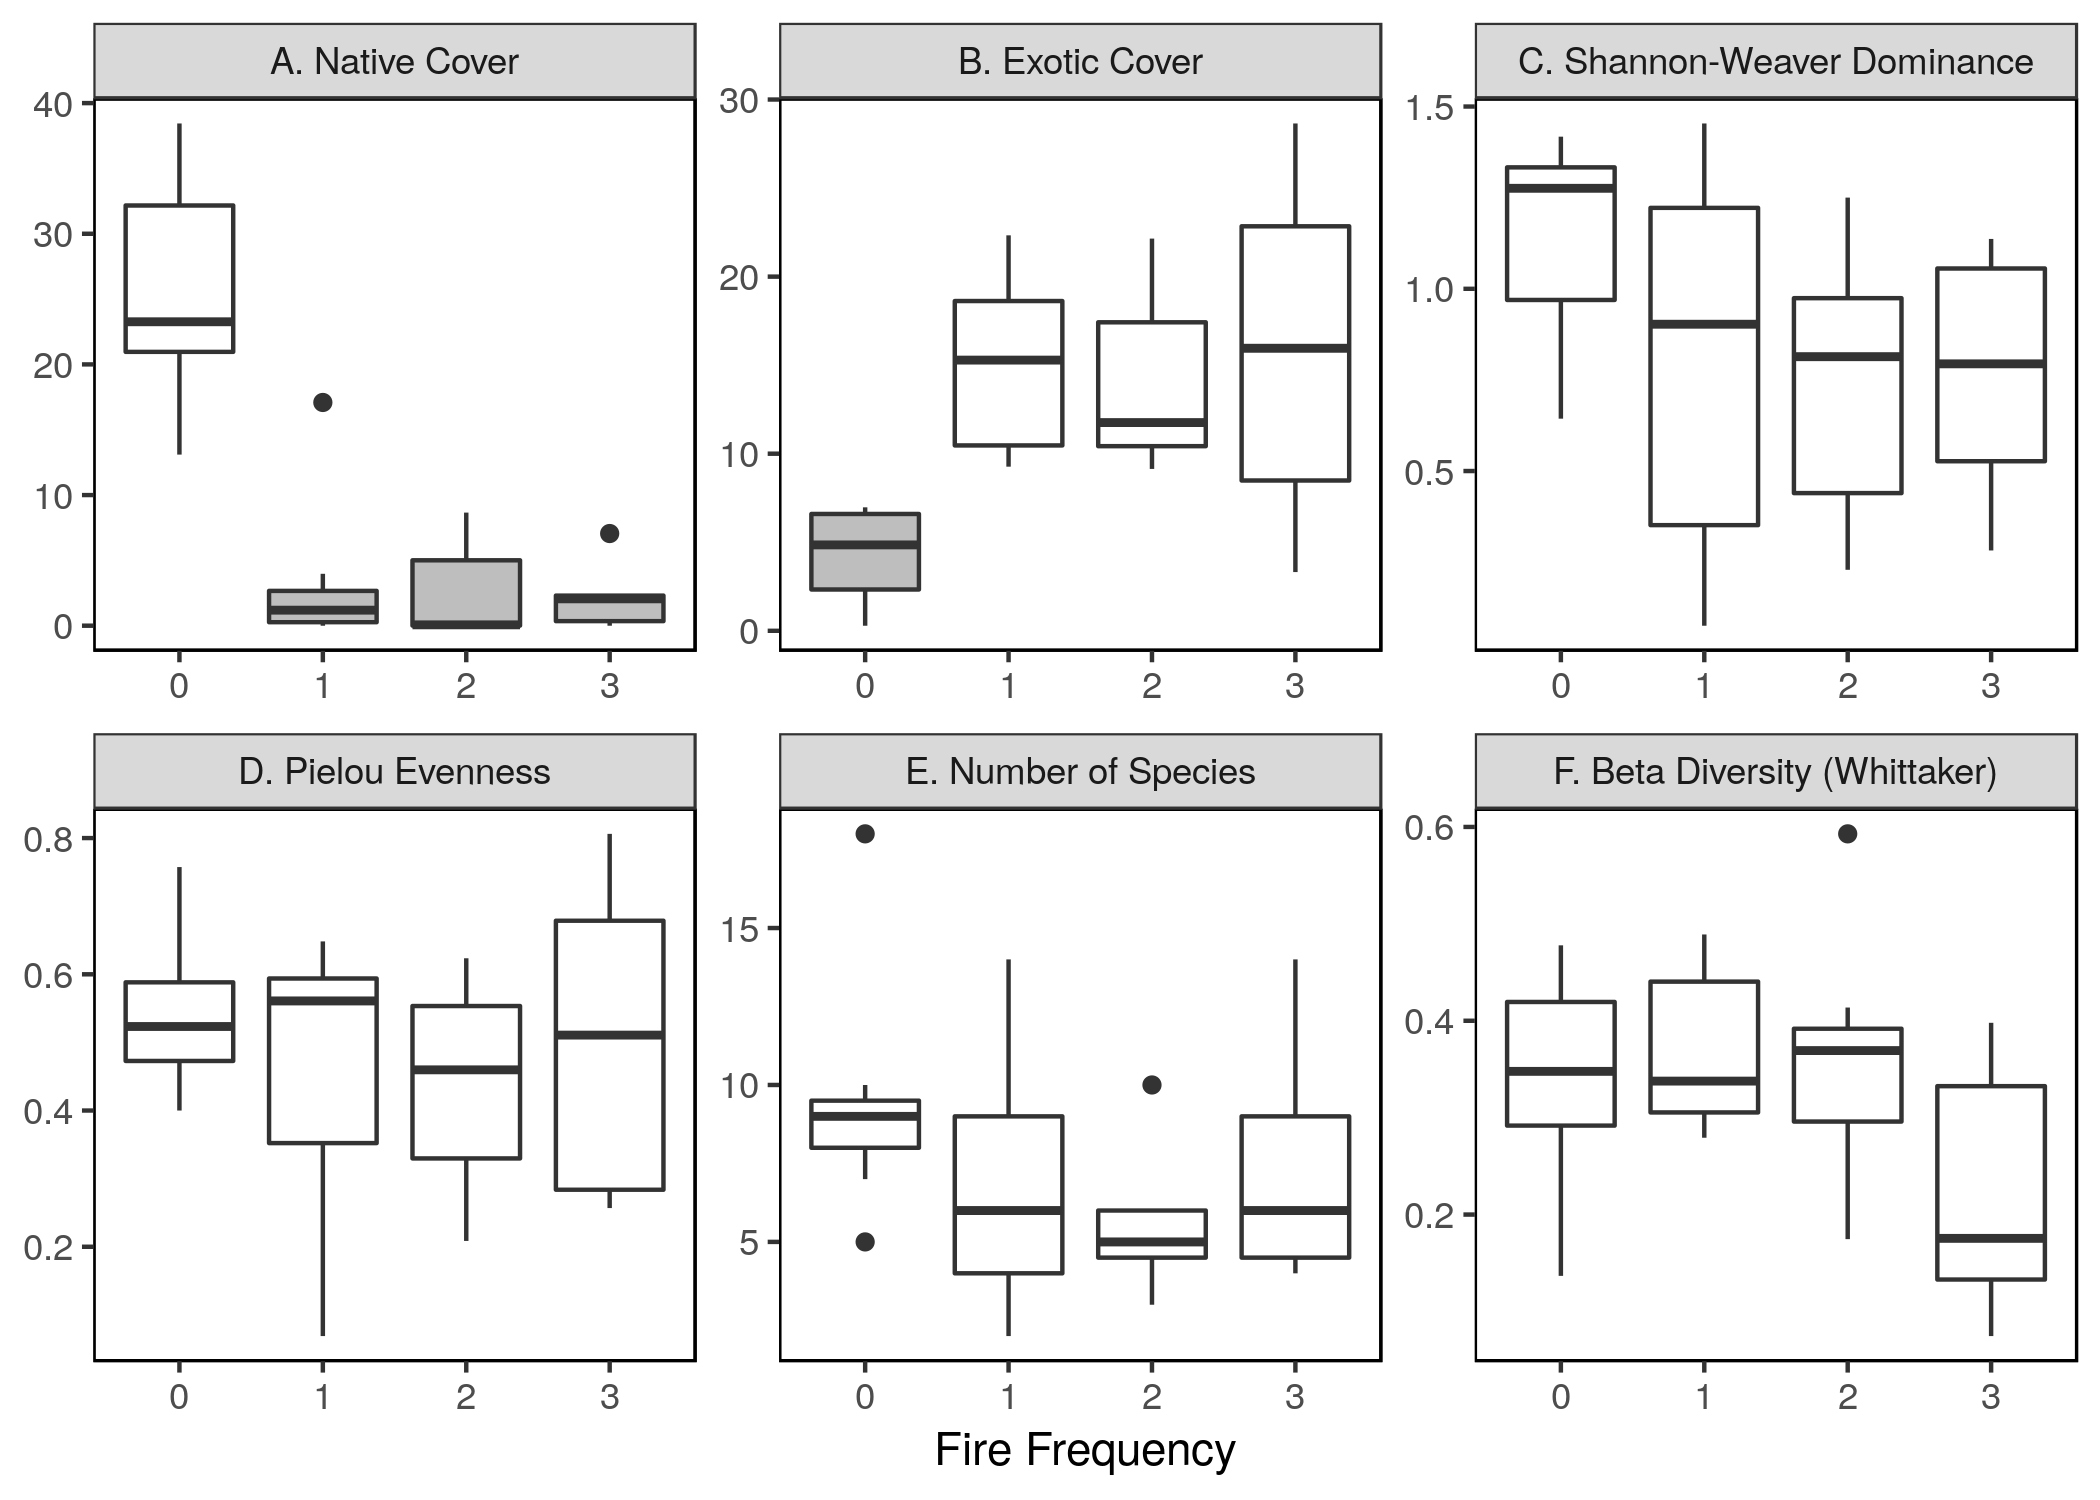
\includegraphics{figures/tukey_plots.png}
    \caption{}
  \end{center}
\end{figure}

\clearpage

\newpage

\begin{figure}
 
  \begin{center}
    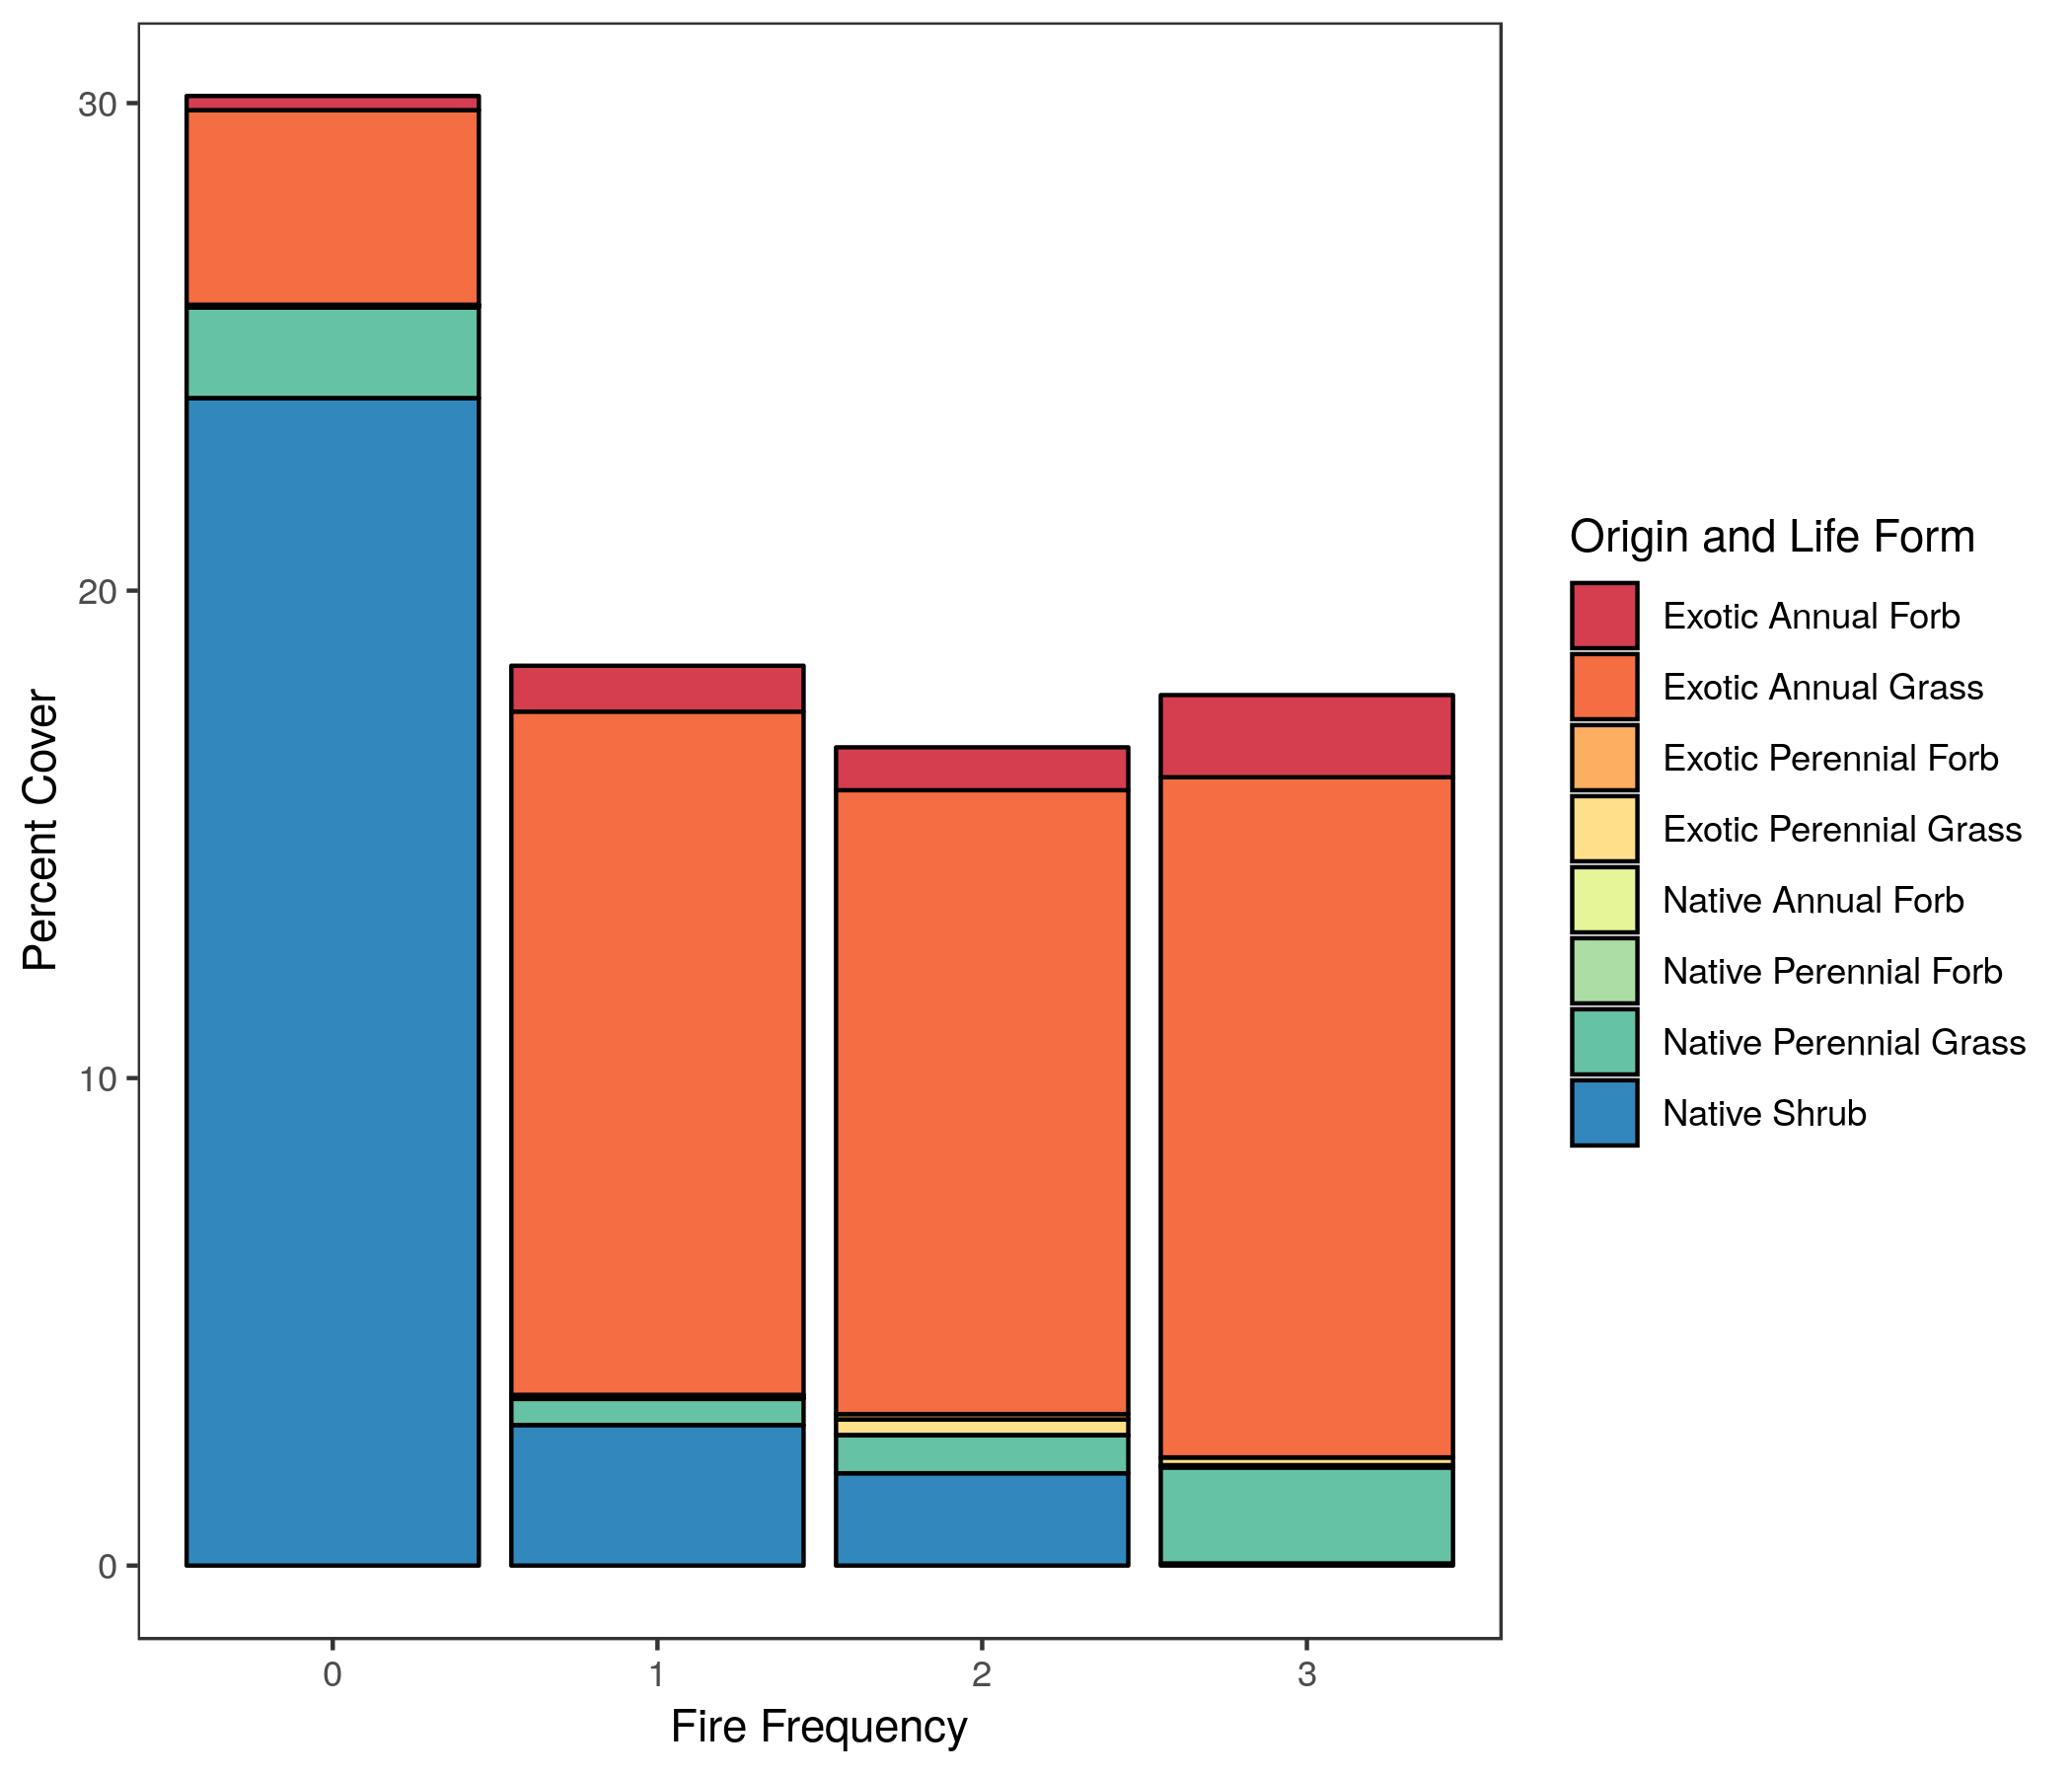
\includegraphics{figures/origin_lf.png}
    \caption{}
  \end{center}
\end{figure}

\clearpage
\newpage

\begin{figure}
 
  \begin{center}
    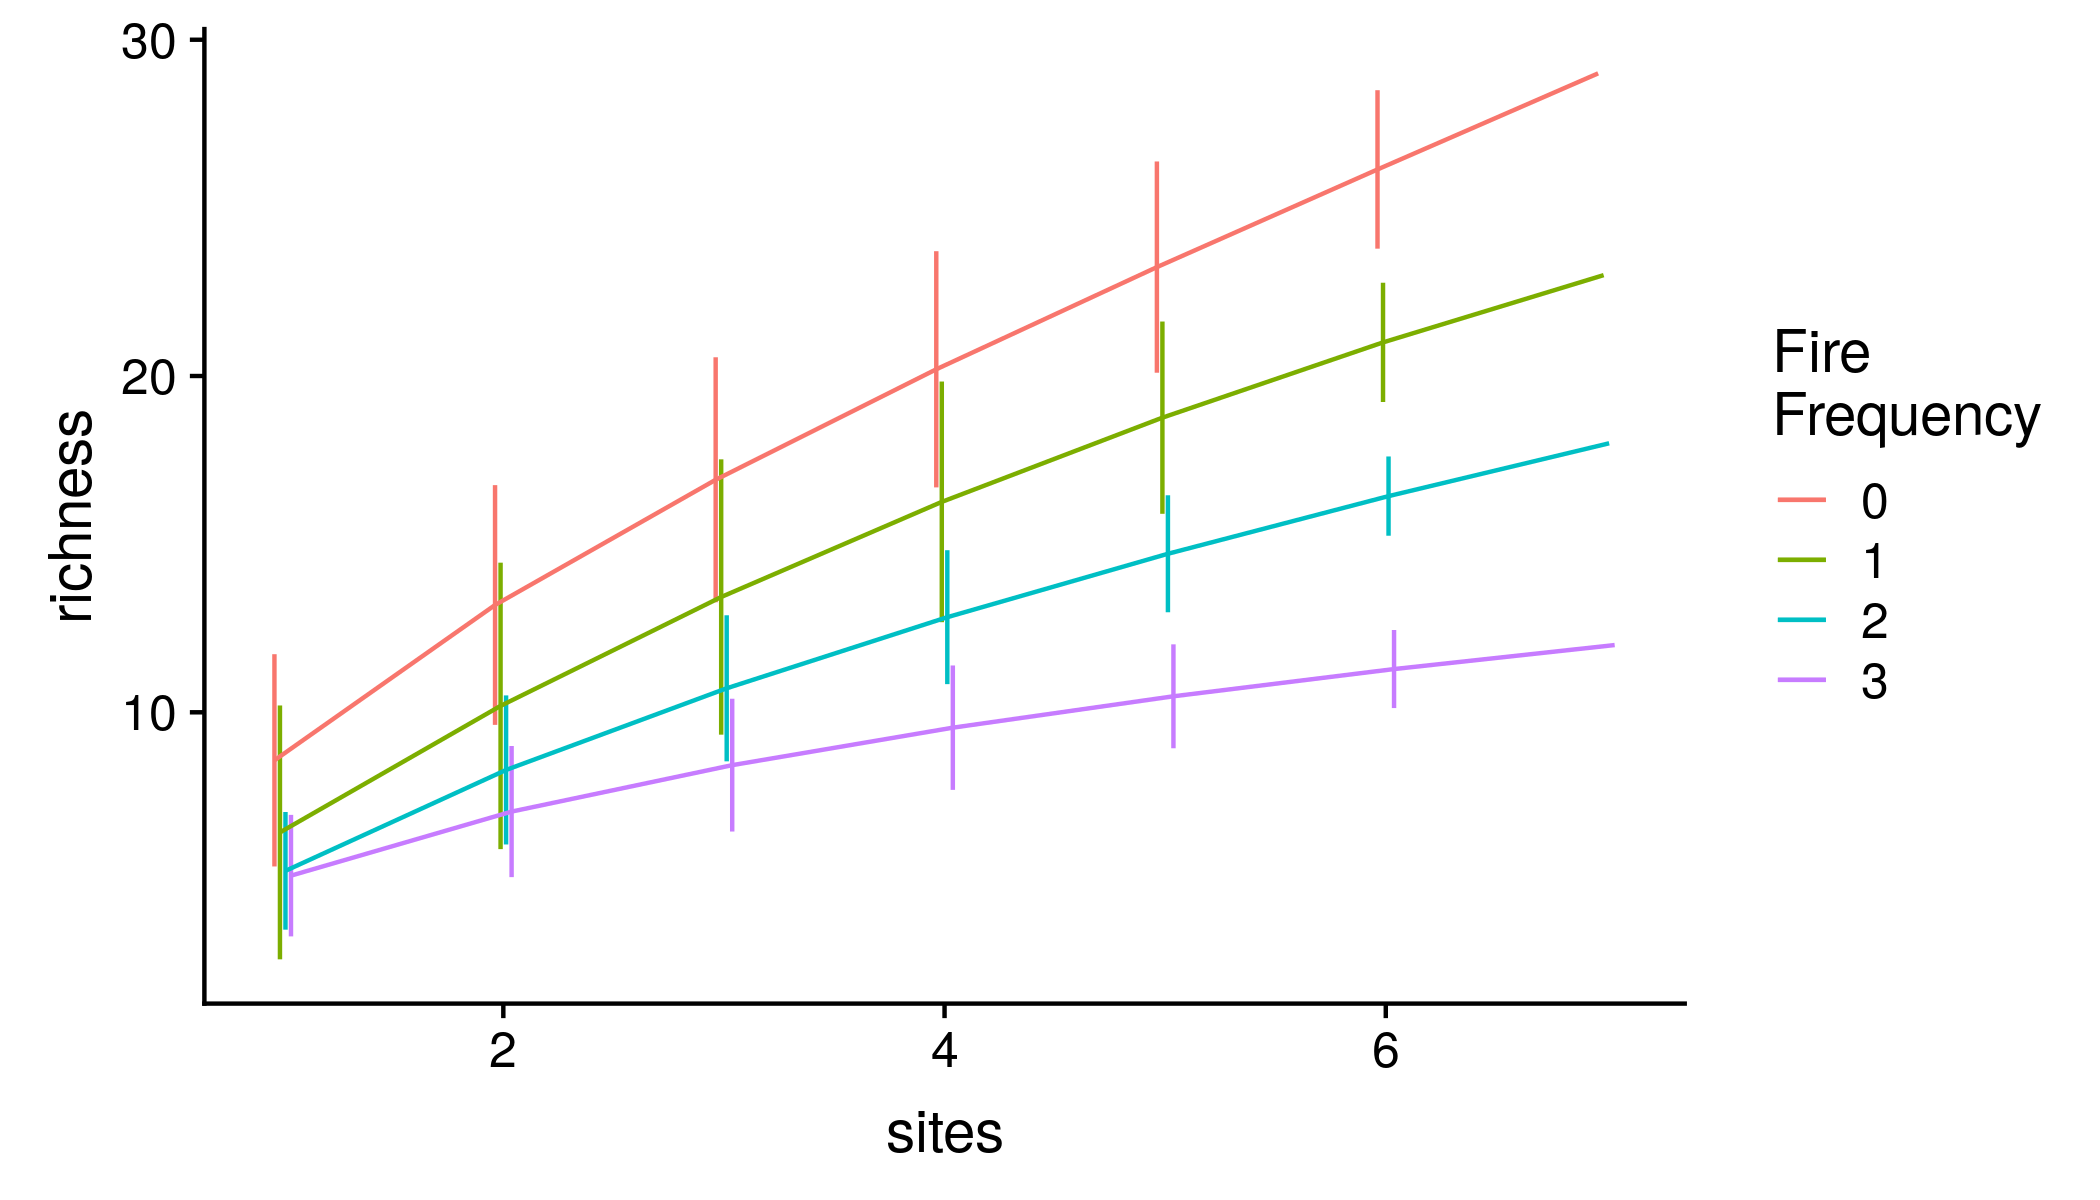
\includegraphics{figures/sac_plot.png}
    \caption{}
  \end{center}
\end{figure}

\clearpage
\newpage

\begin{figure}
 
  \begin{center}
    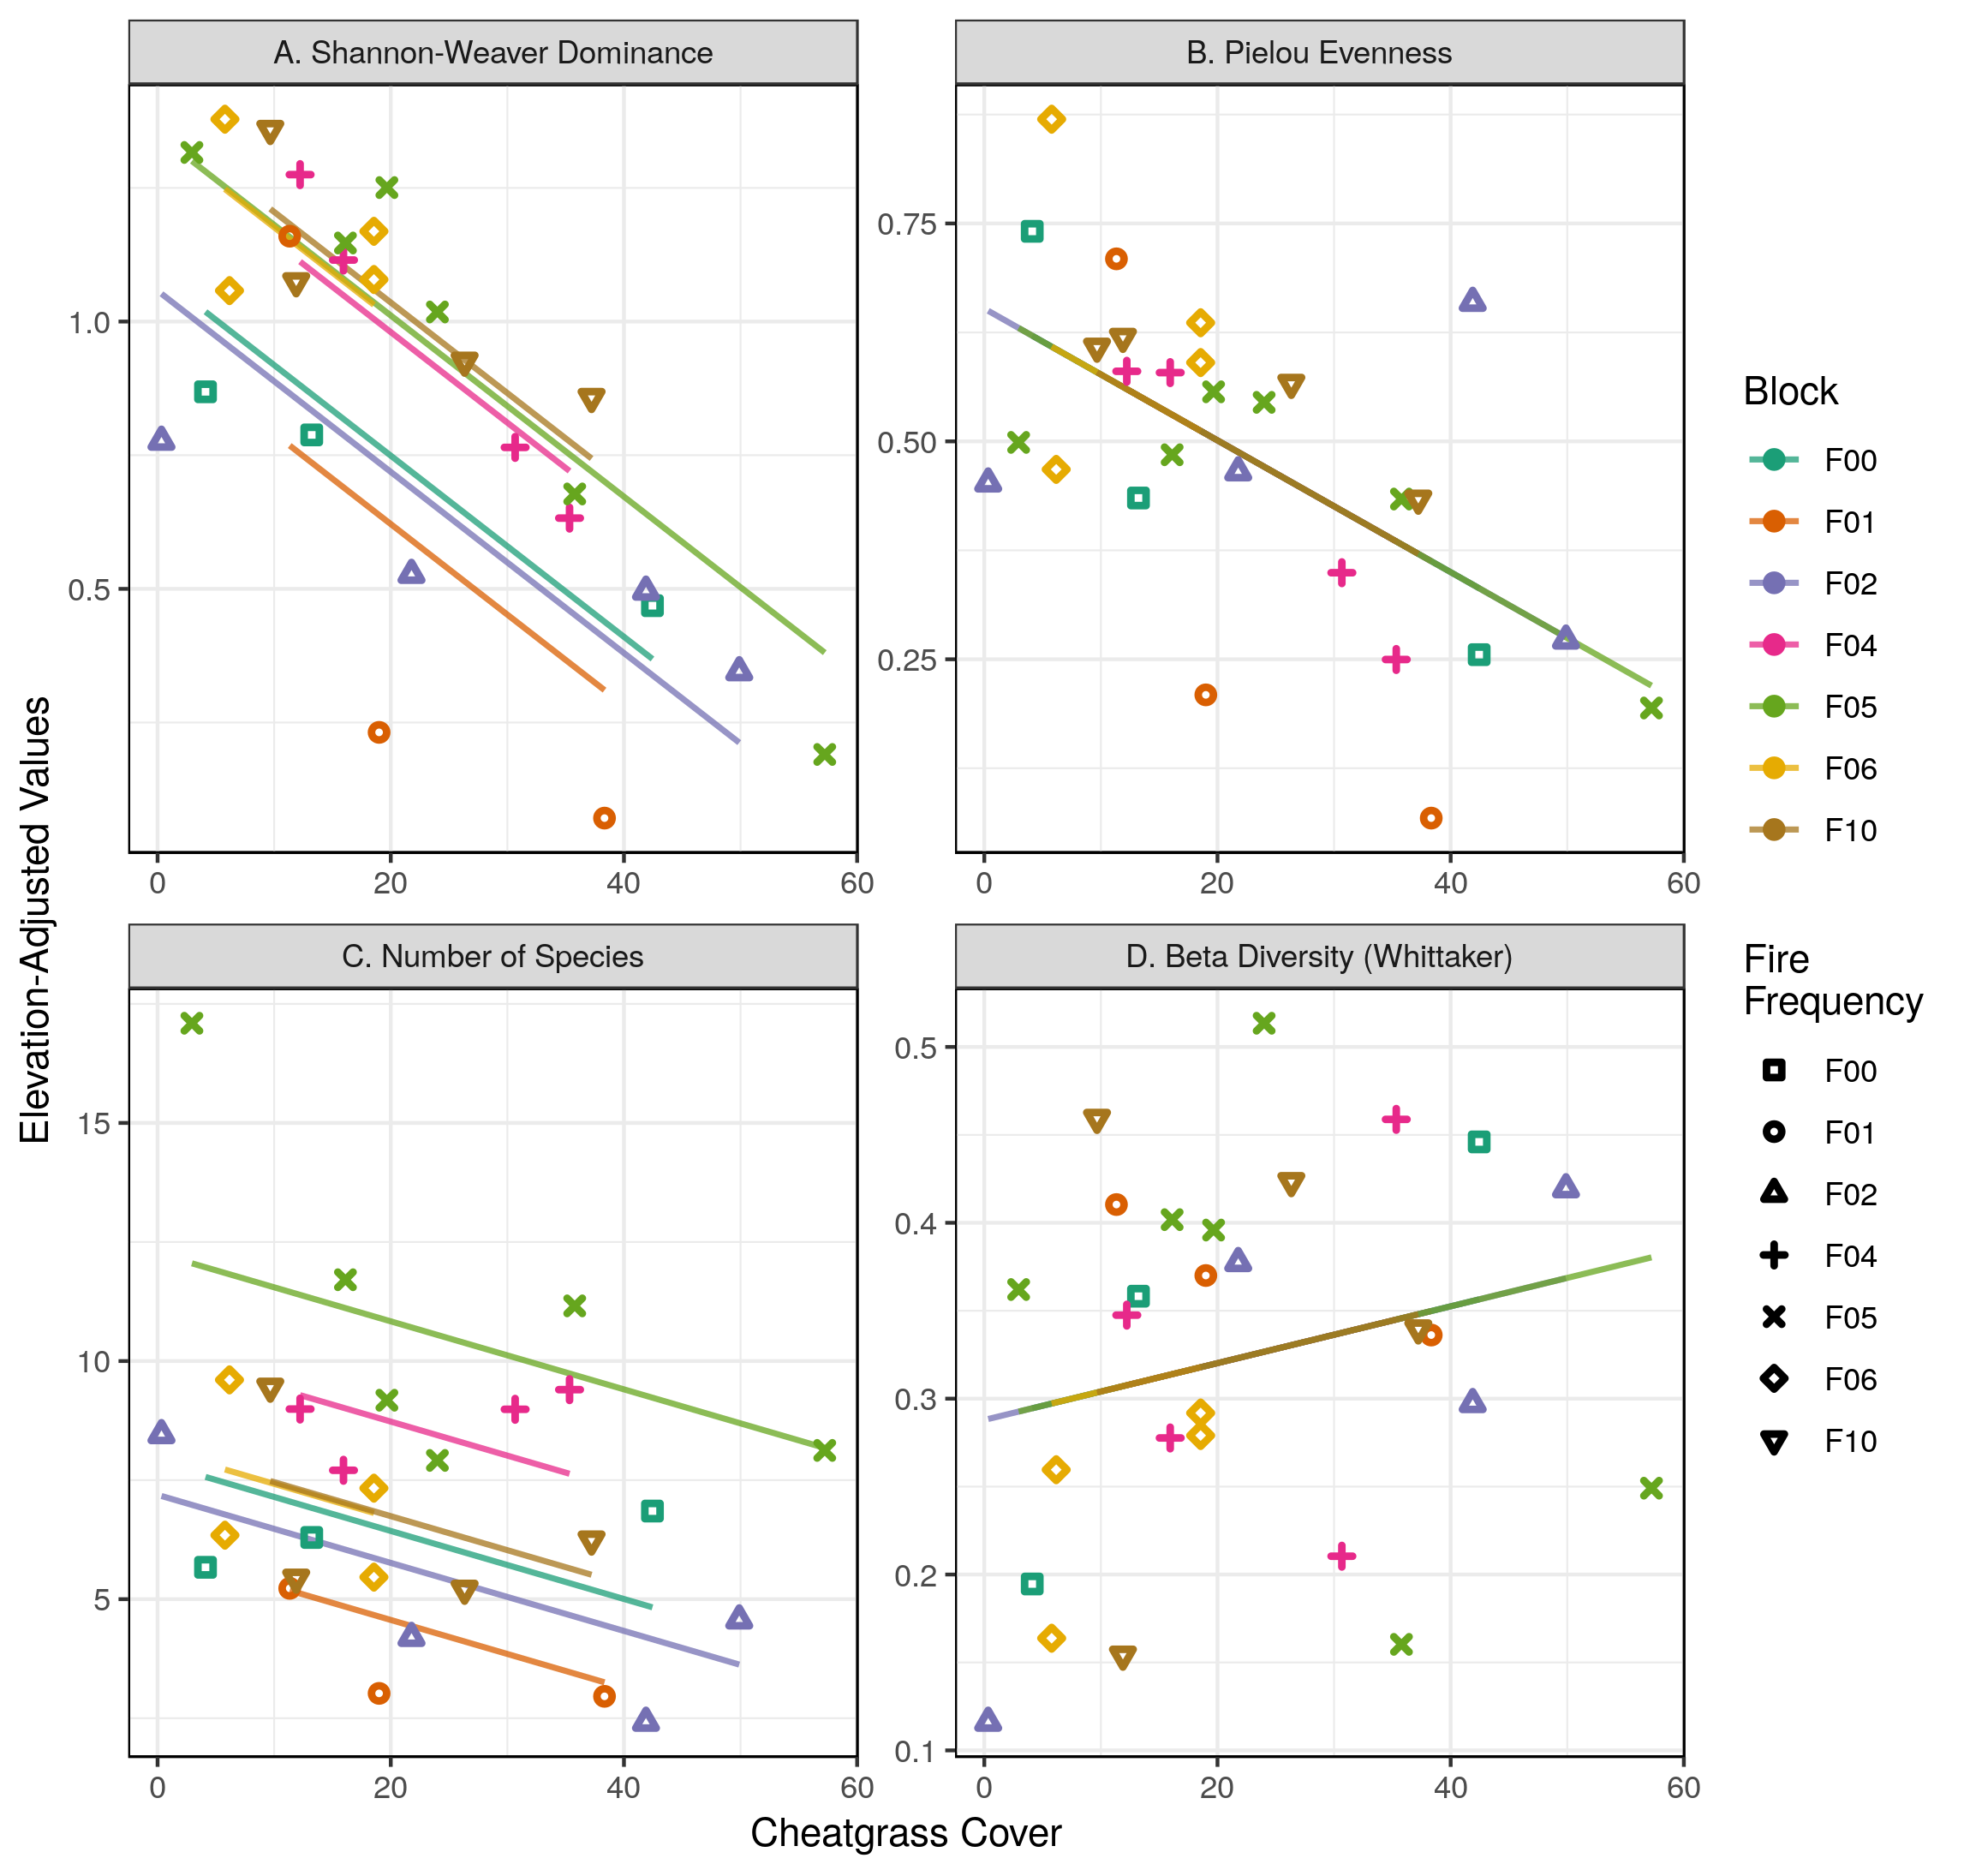
\includegraphics{figures/brte_div.png}
    \caption{}
  \end{center}
\end{figure}


\end{document}
